%%%%%%%% ICML 2021 EXAMPLE LATEX SUBMISSION FILE %%%%%%%%%%%%%%%%%

\documentclass{article}

\usepackage{microtype}
\usepackage{graphicx}
\usepackage{subfigure}
\usepackage{booktabs} % for professional tables
\usepackage{hyperref}
% the following package enables the use of multiline comments:
\usepackage{comment}
\usepackage{amsmath}

% Attempt to make hyperref and algorithmic work together better:
\newcommand{\theHalgorithm}{\arabic{algorithm}}

% Use the following line for the initial blind version submitted for review:
%\usepackage{icml2021}

% If accepted, instead use the following line for the camera-ready submission:
\usepackage[accepted]{icml2021}

% The \icmltitle you define below is probably too long as a header.
% Therefore, a short form for the running title is supplied here:
\icmltitlerunning{Board games group recomendation using metadata}

\begin{document}

\twocolumn[
    \icmltitle{Board games group recomendation using metadata}
    
    % It is OKAY to include author information, even for blind
    % submissions: the style file will automatically remove it for you
    % unless you've provided the [accepted] option to the icml2021
    % package.
    
    % List of affiliations: The first argument should be a (short)
    % identifier you will use later to specify author affiliations
    % Academic affiliations should list Department, University, City, Region, Country
    % Industry affiliations should list Company, City, Region, Country
    
    % You can specify symbols, otherwise they are numbered in order.
    % Ideally, you should not use this facility. Affiliations will be numbered
    % in order of appearance and this is the preferred way.
    \icmlsetsymbol{equal}{*}
    
    \begin{icmlauthorlist}
        \icmlauthor{Eduardo Salinas}{to}
        \icmlauthor{Alfonso Badilla}{to}
        \icmlauthor{Nicolás Gutiérrez}{to}
    \end{icmlauthorlist}
    
    \icmlaffiliation{to}{Department of Computation, Pontificia Universidad Católica de Chile, Santiago, Chile}
    
    \icmlcorrespondingauthor{Eduardo Salinas}{esalinasbarros@uc.cl}
    \icmlcorrespondingauthor{Alfonso Badilla}{alfonso.badilla@uc.cl}
    \icmlcorrespondingauthor{Nicolás Gutiérrez}{njgutierrez@uc.cl}
    
    % You may provide any keywords that you find helpful for describing your paper; these are used to populate the "keywords" metadata in the PDF but will not be shown in the document
    \icmlkeywords{Machine Learning, ICML, Group recommendation, Metadata}
    
    \vskip 0.3in
]

% this must go after the closing bracket ] following \twocolumn[ ...

% This command actually creates the footnote in the first column
% listing the affiliations and the copyright notice.
% The command takes one argument, which is text to display at the start of the footnote.
% The \icmlEqualContribution command is standard text for equal contribution.
% Remove it (just {}) if you do not need this facility.

\printAffiliationsAndNotice{} % otherwise use the standard text.

\begin{abstract}
    In this document we propose a group recommendation system for board games using data from the Board Game Geek website, which includes attributes such as the number of players, average playtime, complexity, and user ratings.
    % todo: agregar explicación groso modo del algoritmo
    The implementation employs Python and the scikit-learn library, offering an efficient and scalable solution for group-based game recommendations.
\end{abstract}

\section{Motivation and state of the art}

Board games have been a popular form of entertainment for centuries, and their popularity has only increased in recent years. Even as digital games have become more prevalent, board games have remained a favorite pastime for many people, and the market for board games has grown significantly giving rise to plataforms such as Board Game Geek\footnote{\cite{boardgamegeek}} (BGG). This website is a popular platform for board game enthusiasts, where users can rate and review games, as well as access information about them.

\subsection{State of the art and related work}

This plataform has a vast amount of data that has been used in the past to create recommendation systems. For example,
github user richengo \yrcite{richengo2024} proposed a recommendation system for board games based on user ratings, using a collaborative filtering approach. However, this approach does not take into account the characteristics of many of the games, that are supposed to be played in groups. As such, we propose a group recommendation system to make recommendations tailored to groups of players.

Another example of group recommendation systems is the work of \cite{group_recommenders_repo}, who proposed a group recommendation system for tourism and movies\footnote{This work is hosted on a github repo and is intended to be used as a basic tutorial.}.
This system uses regular clustering algorithms to group users based on their ratings, such as user k-nearest, item k-nearest and support vector decomposition (SVD), and then recommends movies and touristic locations based on the preferences of the group.

\subsection{Proposal}

We propose a refined version of that last system, using metadata-centric clustering to group board games based on their characteristics, and then recommending games to groups of players based on their summed preferences using the functions detailed on the previous work. This system is designed to be more accuarate than the previous one, as it takes into account the characteristics of the games, and not just the ratings of the users.

\section{Data analysis}

The dataset that will be used for this project\footnote{\cite{board_games_kaggle}}, obtained from the website kaggle, has 10 different files, each one tith different information about board games. The main file is \texttt{user\_ratings.csv}, which contains 19 million rows. Due to the limited processing power of Google Collab and our own local machines, we will use a reduced set of items and users for this work. The other files are:

\begin{itemize}
    \item \texttt{games.csv}: This file contains 22 attributes about the rated games and includes 22,000 different games. Among the attributes, we have aspects such as the game description, which could be evaluated using language models, the year of publication (which distributes as shown in figure \ref{fig:publishYear}), the average rating received, among others.
    \item \texttt{ratings\_distribution.csv}: Contains the total ratings for each board game. In general, these ratings distribute as shown in figure \ref{fig:distribucionRatings}.
    \item \texttt{temes.csv}: Contains the themes of each game as a binary flag. The 50 most common themes can be seen in the graph in figure \ref{fig:tematicasComunes}.
    \item \texttt{mechanics.csv}: Contains the game mechanics as a binary flag. The 50 most common mechanics can be seen in the graph in figure \ref{fig:mecanicasComunes}.
    \item \texttt{subcategories.csv}: Contains the subcategories of each game in binary flag format.
    \item \texttt{artists\_reduced.csv}: Contains information about which artist created a certain game in binary flag format.
    \item \texttt{designer\_reduced.csv}: Contains information about which designer designed a certain game in binary flag format.
    \item \texttt{publishers\_reduced.csv}: Contains information about which companies sell each game in binary flag format.
          
\end{itemize}

\begin{figure}
    \centering
    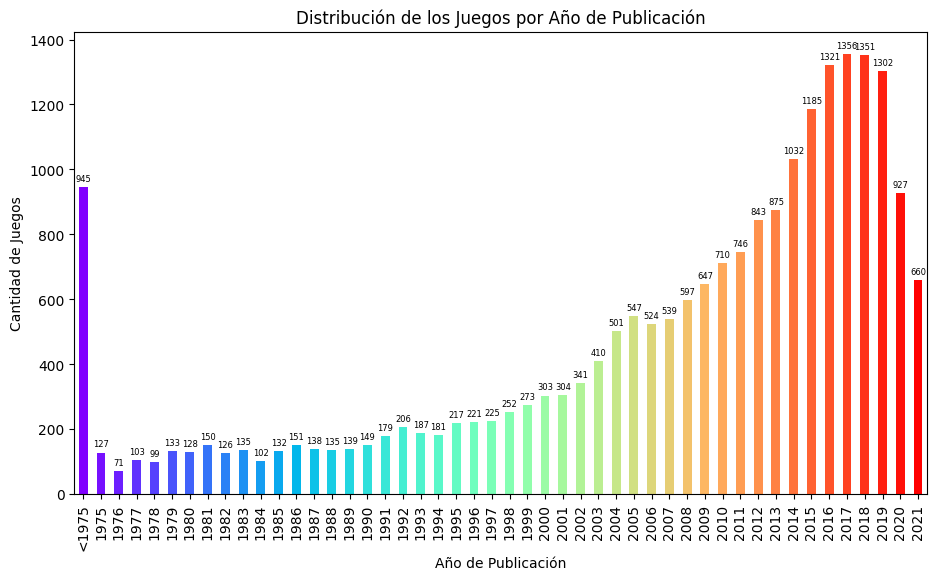
\includegraphics[width=0.9\linewidth]{publishYear.png}
    \caption{Amount of games (y axis) by year of publication(x axis)}
    \label{fig:publishYear}
\end{figure}

\begin{figure}[h]
    \centering
    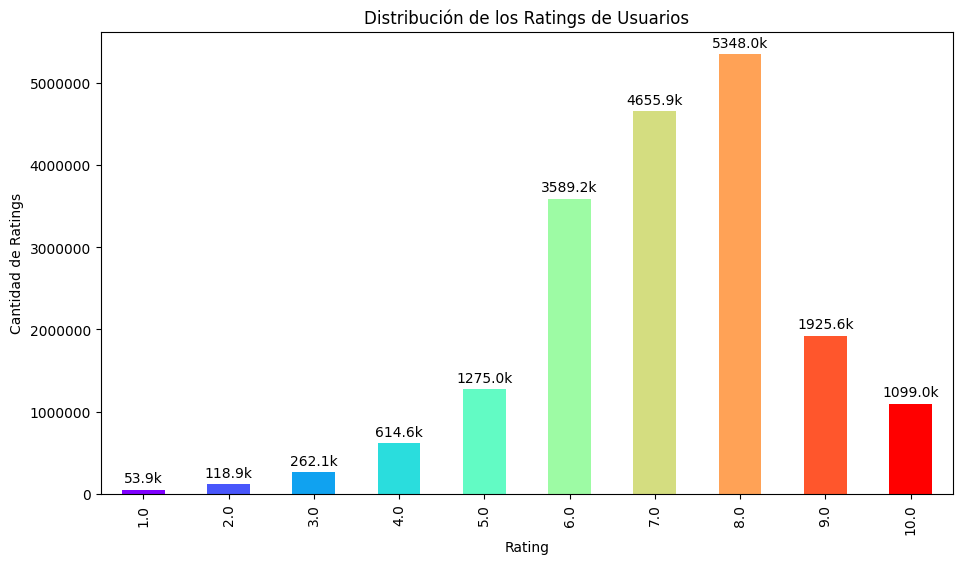
\includegraphics[width=0.9\linewidth]{distribucionRatings.png}
    \caption{Games rating distribution (1-10)}
    \label{fig:distribucionRatings}
\end{figure}

\begin{figure}[h]
    \centering
    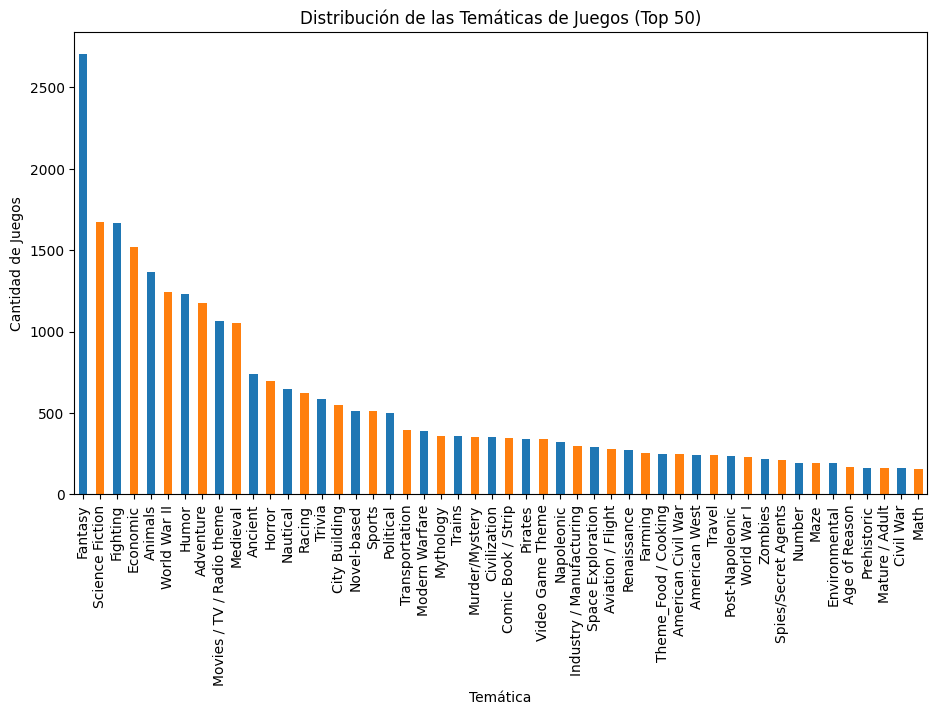
\includegraphics[width=0.9\linewidth]{tematicasComunes.png}
    \caption{Most common game themes on the dataset}
    \label{fig:tematicasComunes}
\end{figure}

\begin{figure}[h]
    \centering
    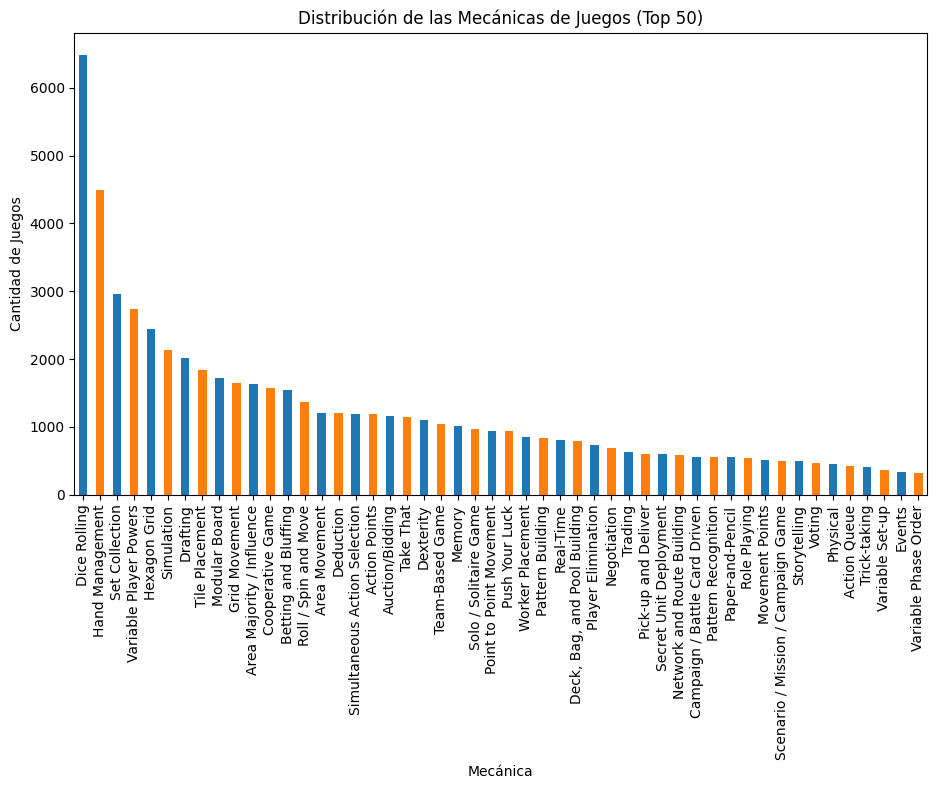
\includegraphics[width=0.9\linewidth]{mecanicasComunes.png}
    \caption{Most common game mechanics on the dataset}
    \label{fig:mecanicasComunes}
\end{figure}

\section{Methodology}

The methodology for this project is divided into three main stages: data preprocessing, group making, and recommendation.

For this project we will use the LightFM library\footnote{\cite{DBLP:conf/recsys/Kula15}} to make the recommendations, which is a Python implementation of a factorization machine for collaborative filtering.

We will also use SVD models from the scikit-learn library\footnote{\cite{scikit-learn}} to compare the results of our model with a more traditional approach, and the most popular model as a baseline. SVD was selected above other models like k-nearest due to its usage as industry standard\footnote{\cite{Roy2022}} and due to taking less time executing.

\subsection{Data preprocessing}
The first stage consists of reducing the dataset. This is important because the amount of data makes it take too long to calculate any meaningful metrics.

Part of the reduction is already done on the dataset by default, since there are no games with less than 20 ratings. Since we are going to also reduce the amount of users, we will delete games further up to 40 ratings, and then pick from 4 different game classes like the ones shown on figure \ref{fig:reviewsPorJuego}.

With that in mind, we will reduce the amount of games to 1500, from the original 22k by taking 375 games from each class.

We will also reduce the amount of users to 15k, from the original $>$300k, first deleting all users with only 1 review. However, the classes will be more complicated to build, since we will be deleting a lot of games, so just making classes like in figure \ref{fig:reviewsPorUsuario} will not be enough.

\begin{figure}[h]
    \centering
    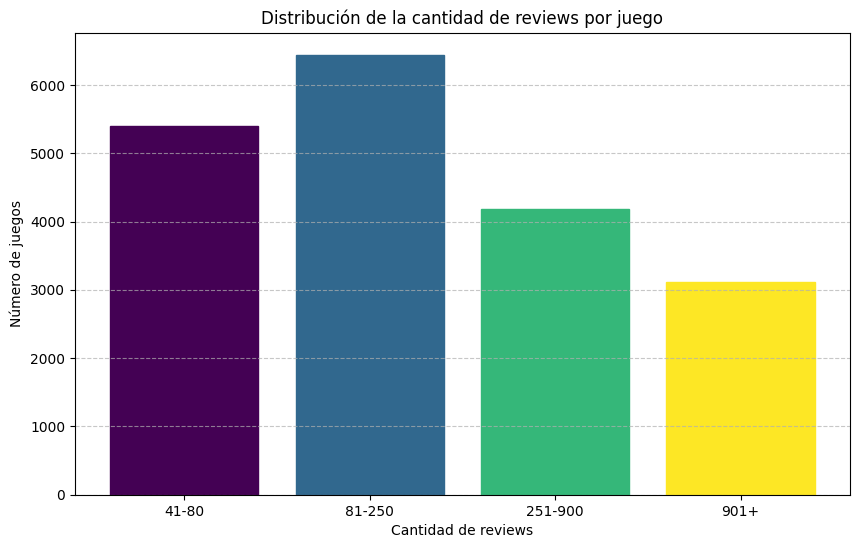
\includegraphics[width=0.9\linewidth]{ReviewsPorJuego.png}
    \caption{Amount of reviews per game}
    \label{fig:reviewsPorJuego}
\end{figure}

\begin{figure}[h]
    \centering
    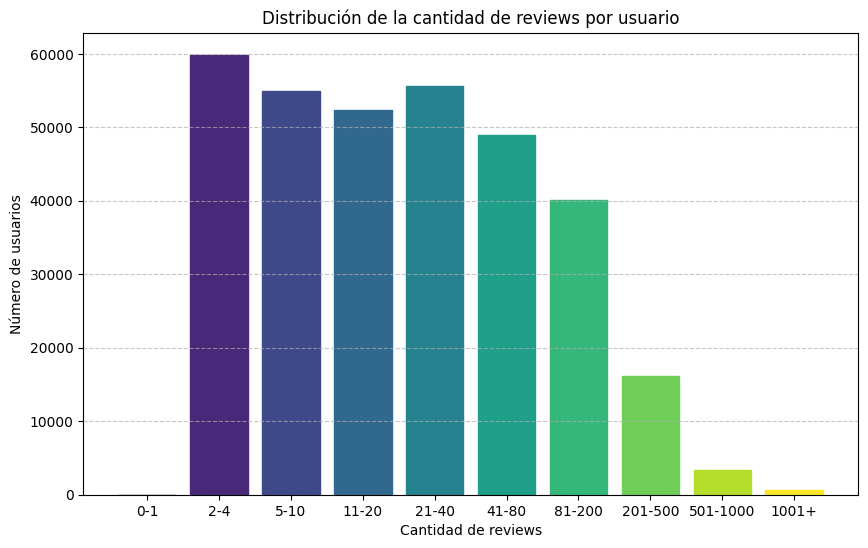
\includegraphics[width=0.9\linewidth]{reviewsPorUsuario.png}
    \caption{Amount of reviews per user (full dataset)}
    \label{fig:reviewsPorUsuario}
\end{figure}

To do that, we will have to make the graph after selecting the games from each class. This graph can be seen in figure \ref{fig:reviewsPorUsuario2}, and as seen on that figure, the classes have shifted due to less reviews overall. We will then make 3 classes as shown, and select 5k users from each class. Note that we will not select users with less than 3 reviews.

\begin{figure}[h]
    \centering
    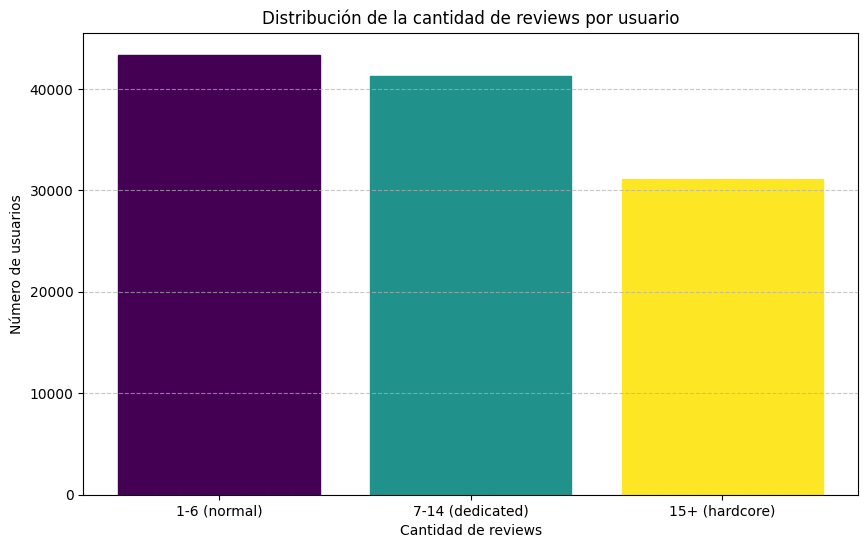
\includegraphics[width=0.9\linewidth]{reviewsPorUsuario2.png}
    \caption{Amount of reviews per user (1500 items)}
    \label{fig:reviewsPorUsuario2}
\end{figure}

The final dataset will have 1500 games and 15k users, and will be used for the rest of the project. The dataset will be split into a training and a test set, with 75\% of the data being used for training and 25\% for testing.

The final amount of reviews per user and per game can be seen in figure \ref{fig:reviewsPorUsuarioFinal} and figure \ref{fig:reviewsPorJuegoFinal} respectively.

\begin{figure}[h]
    \centering
    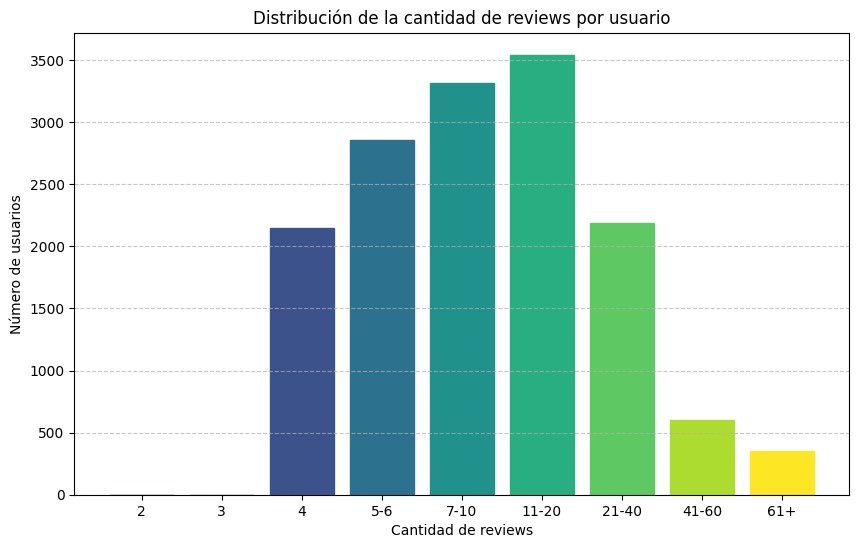
\includegraphics[width=0.9\linewidth]{reviewsPorUsuarioFinal.png}
    \caption{Amount of reviews per user (after full reduction)}
    \label{fig:reviewsPorUsuarioFinal}
\end{figure}

\begin{figure}[h]
    \centering
    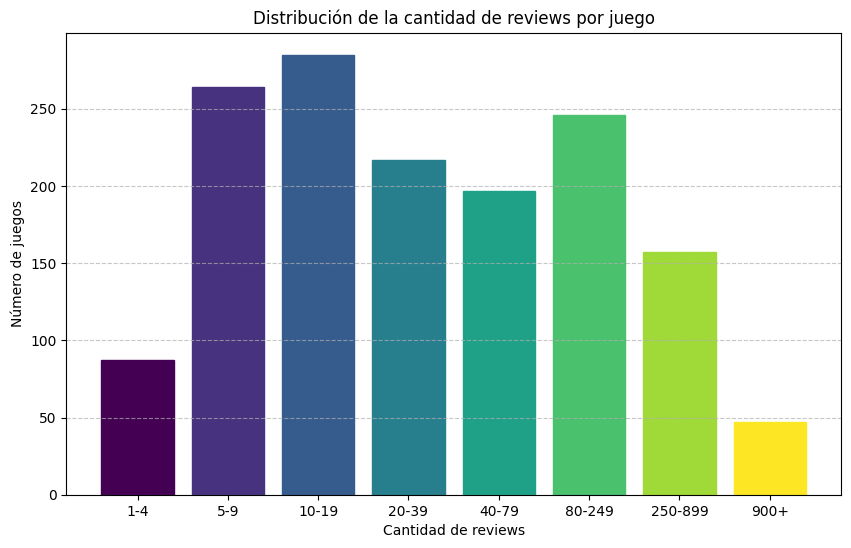
\includegraphics[width=0.9\linewidth]{ReviewsPorJuegoFinal.png}
    \caption{Amount of reviews per game (after full reduction)}
    \label{fig:reviewsPorJuegoFinal}
\end{figure}

With this, we expect to make a more efficient solution for group-based game recommendations, so that it can run with regular hardware.

\subsection{Group making}

% Insertar referencia y citar apropiadamente el trabajo.
The second stage consists of grouping the users based on their characteristics by using a correlation matrix. The function used is an adaptation of the one used in the work of \cite{group_recommenders_repo}. This function is used to calculate the similarity between users based on their ratings, and then group them based on that similarity.

To assemble groups by similarity, we use the Pearson product-moment correlation coefficients matrix. In order to do this, a matrix with users by rows and items by columns is built, in which the entry $i,j$ is the rating that the user $i$ gave to item $j$, every item that is not rated is rated as 0.

From that matrix, we calculate the coefficient matrix where the entry $i,j$ is $$\frac{C_{ij}}{\sqrt{C_{ii}C_{jj}}}$$ with $C_{ij}$  the covariance between user $i$ and user $j$.

The groups are then formed by selecting the users with the highest correlation coefficients. The number of groups is determined by the user, and the number of users per group is also determined by the user. For this work, we will use as many groups as possible with 4 users each (as it is the most common maximum of players for a given game in this dataset, as seen on figure \ref{fig:output}).

\begin{figure}[h]
    \centering
    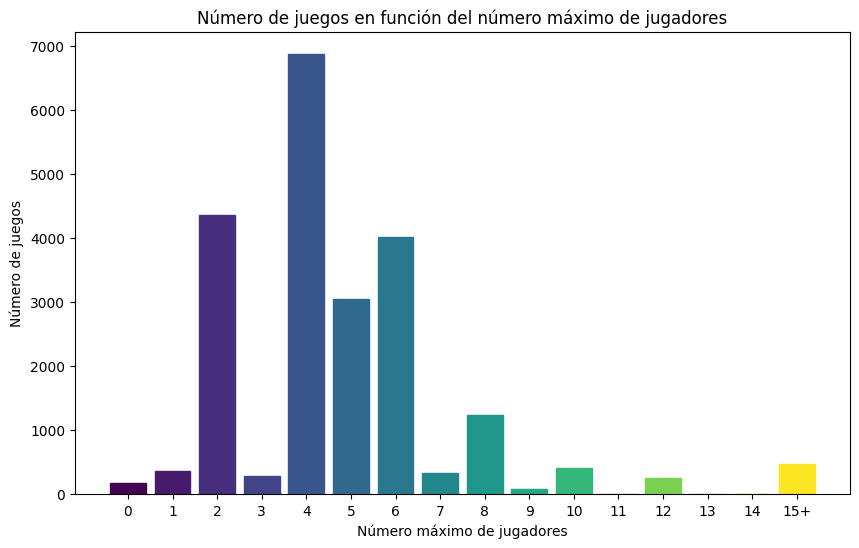
\includegraphics[width=0.9\linewidth]{output.png}
    \caption{Most common number of max players}
    \label{fig:output}
\end{figure}

\subsection{Recommendation}
The third stage consists of recommending games to groups of players based on their preferences. Since the recommendations are supposed to be made to groups, the preferences of the group are calculated using a variety of methods, that can be described as follows:
\begin{enumerate}
    \item Simple average: The preferences of the group are calculated as the simple average of the preferences of the individual players based on a top-100 recommendation list prior to the group formation. This can be done with the following formula:
          \begin{equation}
              \text{avg\_score\_item} = \frac{\sum_{i=1}^{n} \text{user\_rating}_i}{n}
          \end{equation}
          with $n$ being the number of users in the group, and $u_i$ being the rating of the $i$-th user given an item.
          % \item Least misery: The preferences of the group are calculated as the minimum of the preferences of the individual players.
          % \item ... % asegurarse que esto está al día con lo que presentemos al final del trabajo
\end{enumerate}

Given the method explained above, we assign the score to each of the items in the top-100 recommedation list of each user on a group. Then we create a new list of items combining the top-100 recommendation lists of each user on a group, and we extract the top-n items with the highest average scores. Note that for this to work properly, if two users have a matching item in their top-100 recommendation list, the item will only be included as the sum of the average rankings by the users in the group.



\section{Results}

To evaluate the results of our model, we will compare it to most popular as a sanity check and to SVD applied to the same dataset and groups. % Agregar AGREE si logramos hacerlo funcionar ahora que tenemos menos datos. 

The metrics that will be used to evaluate the performance of each model are the following:

\begin{itemize}
    \item Precision@k: This metric measures the proportion of recommended items that are relevant to the user, where relevance is defined as the items that the user has interacted with.
    \item Recall@k: This metric measures the proportion of relevant items that are recommended to the user.
    \item nDCG@k: This metric measures the normalized discounted cumulative gain at k, and is used to measure the quality of the recommendations.
    \item Relevance Score: This metric evaluates how relevant the recommendations are to the user, providing an indication of the recommendation quality.
    \item Diversity: This metric assesses the variety of the recommendations, ensuring a wide range of different items are suggested.
    \item Novelty: This metric measures how new or unexpected the recommendations are to the user, contributing to the overall recommendation quality.
    \item Fairness: This metric evaluates the fairness of the recommendations, ensuring that the recommendations are unbiased and equitable.
    \item Serendipity: This metric measures the likelihood of the recommendations to pleasantly surprise the user, enhancing the user experience.
\end{itemize}

For each metric, we used a cumulative avarage of the results of 300 different group formations, on which we applied the common formulas for each metric. Meaning that, for each group, we calculated all of the metrics mentioned above, then we added them and divided by the number of groups.

As is shown on tables \ref{tab:resultados-modelos} and \ref{tab:resultados-modelos-similar}, the LightFM model outperforms the other models in almost all metrics. This is what we where looking for in this work, that it gives better metrics since its using not only user-item interactions but also metadata to make recommendations. 
The metadata recommendation allows for the model to recommend similiar items to two or more users that have similar preferences even if they have not interacted with any items in common. This is specially helpful when 
making groups recommendations, because it allows for greater diversity and novelty and creates a more personalized group experience.

One aspect of the recommendations that is worth mentioning is that the LightFM model is capable of superior results with more diversity. This means that all groups will get recommended different games, but they are tailored to the preferences of each user on a group. This in hand increases the novelty and the serendipity of the recommendations, creating more unique experiences for the users.

For each different group formation, the results are mostly the same. This is to be expected, since the group formation is based on the preferences of the users, and the recommendations are made based on the preferences of the group. Not on the preferences of the individual users. This is a good sign, beacuase it shows that the model does not overfit to any group formation and it is able to make recommendations based on the preferences of the group.

However, for new users, the results might not be as expected. The user needs to create user-item interactions in order to get proper recommendations. Untill then, the model should be able to recommend the most popular items, which are the most likely to be relevant to the user according to the very low information the model has.

\begin{table}[]
    \centering
    \begin{tabular}{|l|l|l|l|}
        \hline
        \textbf{Statistic} & \textbf{LightFM} & \textbf{SVD} & \textbf{Most Popular} \\ \hline
        Precision@5        & 0.3660           & 0.2020       & 0.3010                \\
        Recall@5           & 0.0942           & 0.0520       & 0.0766                \\
        nDCG@5             & 0.6232           & 0.4762       & 0.5903                \\
        Relevance Score    & 2.76             & 1.59         & 2.32                  \\
        Diversity          & 0.03             & 0.01         & 0.01                  \\
        Novelty            & 5.89             & 8.52         & 5.70                  \\
        Fairness           & 0.60             & 0.72         & 0.66                  \\
        Serendipity        & 4.51             & 2.80         & 3.63                  \\ \hline
    \end{tabular}
    \caption{Random groups recomendation results}
    \label{tab:resultados-modelos}
\end{table}

\begin{table}[]
    \centering
    \begin{tabular}{|l|l|l|l|}
        \hline
        \textbf{Statistic} & \textbf{LightFM} & \textbf{SVD} & \textbf{Most Popular} \\ \hline
        Precision@5        & 0.3350           & 0.2040       & 0.3240                \\
        Recall@5           & 0.0821           & 0.0498       & 0.0749                \\
        nDCG@5             & 0.5722           & 0.4736       & 0.5474                \\
        Relevance Score    & 2.57             & 1.62         & 2.48                  \\
        Diversity          & 0.04             & 0.01         & 0.01                  \\
        Novelty            & 5.99             & 8.60         & 5.70                  \\
        Fairness           & 0.63             & 0.72         & 0.64                  \\
        Serendipity        & 4.61             & 2.75         & 4.06                  \\ \hline
    \end{tabular}
    \caption{Similar groups recommendation results}
    \label{tab:resultados-modelos-similar}
\end{table}

\section{Conclusions}

In this work, we proposed a group recommendation system for board games using metadata from the Board Game Geek website. The system uses a LightFM model to make recommendations based on the preferences of the group. 

Our system outperforms traditional recommendation models, such matrix factorization (SVD), in terms of key metrics like Precision, Recall, nDCG, Diversity, and Serendipity. By incorporating metadata — including attributes like game mechanics, themes, and complexity — our model provides more personalized and diverse recommendations.

The results are consistent across different group formations, showing that the model is able to make recommendations based on the preferences of the group, and not on the preferences of the individual users. This is a key advantage of our system, as it ensures that the recommendations are tailored to the group as a whole, rather than to individual users.

The results also highlight the value of metadata in enhancing recommendation accuracy, ensuring greater variety and novelty in the suggested games, and improving the overall user experience. Our method not only improves the quality of recommendations but also addresses the challenge of recommending games for groups with diverse preferences. 

This work shows that metadata-based group recommendation systems can be an effective way to make recommendations for board games, especially with low computational power available. The robustness and scalability of the proposed system indicate its potential for application in other domains requiring group-based recommendations, such as tourism, movies, or event planning, assuming the metadata is available.

\section{Future work}

Since this project was done with a reduced dataset, the obvious step would be to scale it up to the full dataset or at least a bigger portion of it with improved computation power. This would allow for more accurate results and a more robust set of models.

Another step would be to improve the group formation algorithm, as it is currently based on the preferences of the users, and not on the characteristics of the games they play (it does not use the available metadata). This could be done by using a clustering algorithm to group the games based on their characteristics, and then grouping the users based on the games they have interacted with. Future work could also use a hybrid approach, where part of how the groups are formed is random and another part is based on the similarity of the users.

Additionally, a notable drawback of this work is the lack of inclusion of the baseline "AGREE" recommended by the course instructors of IIC3633. Since the dataset selection process was finalized late in the development of this work, this implementation was not completed.

Finally, there is exploration to do regarding the use of the least misery and dictatorship aggregation functions, as well as the use of other aggregation functions that could be more suitable for group recommendations. This could be done by comparing the results of the different aggregation functions and selecting the one that provides the best recommendations. This barely didnt make it into the project, and could easily be implemented in the future.

\bibliography{main}
\bibliographystyle{icml2021}


\end{document}

